%%%%%%%%%%%%%%%%%%%%%%%%%%%%%%%%%%%%%%%%%%%%%%%%%%%
%
%  New template code for TAMU Theses and Dissertations starting Fall 2016.  
%
%
%  Author: Sean Zachary Roberson
%  Version 3.17.09
%  Last Updated: 9/21/2017
%
%%%%%%%%%%%%%%%%%%%%%%%%%%%%%%%%%%%%%%%%%%%%%%%%%%%

%%%%%%%%%%%%%%%%%%%%%%%%%%%%%%%%%%%%%%%%%%%%%%%%%%%%%%%%%%%%%%%%%%%%%%
%%                           SECTION I
%%%%%%%%%%%%%%%%%%%%%%%%%%%%%%%%%%%%%%%%%%%%%%%%%%%%%%%%%%%%%%%%%%%%%


\pagestyle{plain} % No headers, just page numbers
\pagenumbering{arabic} % Arabic numerals
\setcounter{page}{1}


\chapter{\uppercase {Introduction and Literature Review}}

 The growing use of fiber-matrix composite materials as both a decorative and functional material has also increased the need to better understand these materials in all of their forms. From unidirectional ply composites to intricate woven textile composites, the need for understanding material properties and mechanics for these composites has never been higher. In order to gain a more intimate understanding of the mechanical response for these composites, research turned towards computational models and simulations that were validated with experimental data. As these models became more accurate, understanding of both mechanical response and damage initiation increased. The use of computational models and analysis is now a fundamental aspect of most engineering and scientific research, and can been seen in use as far as early undergraduate studies.


\section{Motivation}

The motivation for this work comes from the desire to more correctly and realistically model fiber-matrix composite materials. Substantial experimental and computational research has been conducted on unidirectional ply composite as well as experimental research on textile woven composites. However, there is still a need for non-idealized textile composite geometries for computational analysis. The use of these geometries range from verification of computational models to insight into damage initiation and growth. 

While there exists multiple software that can generate these geometries, the process (to be discussed later) can result is surface meshes of the geometries can be incompatible and have inter-penetrations between them. A generalized solution to this issue could prove useful to future research in this area.

\section{Woven Textile Composite Simulation}

One method to creating more realistic woven geometries is to simulate the process that manufactures employ to create the fabrics \cite{Wang_Sun1}. The process begins by simulating bundles of fibers as "yarns". These yarns  are made up of digital elements (cylindrical bars connected by friction-less pins) chained together. Each bar is given a stiffness in the longitudinal direction that amounts to a large value which eliminates yarn stretching. Then, a finite element style contact problem is solved where pins between two yarns can create contact forces between each other as well as friction forces. The result is realistic interactions between the digital chains. \cite{Wang_Sun1} 

The result is fiber bundle cross sections that are similar to micro-CT scans from actual woven specimens, shown in Figure 1.1, from \cite{Wang_Sun1}.

\begin{figure}[ht]
\centering
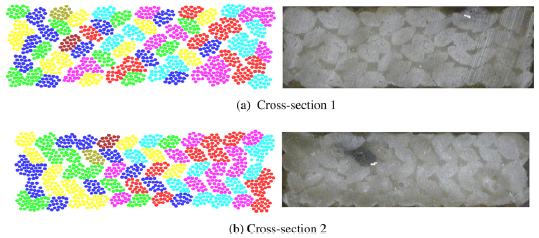
\includegraphics[scale=0.95]{CrossSections.png}
\caption[Simulated vs. Actual Fiber Bundle Cross Sections]{Simulated (left (a) and (b)) vs. Actual Fiber Bundle Cross Sections}

\end{figure}


While there is possibly other software that can accomplish this level of similarity between simulation and reality, only two were explored. The first is Digital Fabric Mechanics Analyzer (DFMA) from Kansas State, overseen by Youqi Wang and students. The other is Virtual Textile Morphology Suite (VTMS), developed by Eric Zhou at AFRL. It should be noted that Eric Zhou is a former student of Youqi Wang and is cited in a previous paper \cite{Wang_Zhou1}.

It is from VTMS that the base geometry and surface mesh that is used in this study originates. Figure 1.2 shows the process visually. The surface inter-penetrations come as a result from the geometries shown in Figure 1.2.d).

\begin{figure}
\centering
\begin{subfigure}{.45\textwidth}
  \centering
  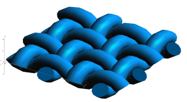
\includegraphics[width=.8\linewidth]{VTMS_Tubes.png}
  \caption{Generic Approximation of Woven Pattern}
\end{subfigure}
\begin{subfigure}{.45\textwidth}
  \centering
  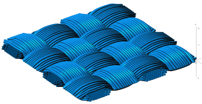
\includegraphics[width=.8\linewidth]{VTMS_Textile.png}
  \caption{Yarn Representation of Pattern}
\end{subfigure}

\begin{subfigure}{.45\textwidth}
  \centering
  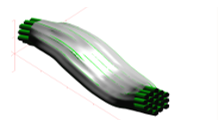
\includegraphics[width=.8\linewidth]{VTMS_Wrapped.png}
  \caption{Surface Approximation of Yarn Bundles}
\end{subfigure}
\begin{subfigure}{.45\textwidth}
  \centering
  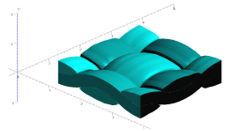
\includegraphics[width=.8\linewidth]{VTMS_Surface.png}
  \caption{Volume Model Derived from Surfaces}
\end{subfigure}
\caption{Evolution of Weave Textile Geometry}
\end{figure}

The reasoning behind creating surface and volume approximations (Figure 1.2.c and d) is that the computational cost of analyzing many bundles that represent woven fibers is very high. Instead, researchers currently are content with using a surface or volume approximation and applying material properties found in experiments.

\section{Introduction to Interpenetration Regions}

Once a surface representation is created, surfaces in close proximity have the ability to penetrate into each other, as shown in Figure 1.3. The arrows in Figure 1.3.b) indicate regions where one surface mesh is penetrating into the other. Physically, the two surfaces would come into contact and create some form of surface. This reaction is not represented here because the surfaces are created after the simulation process is done. These inter-penetrations represent the error in approximating the yarn bundles as a surface to apply homogenized properties to for analysis. Here in lies the focus of this study. Traditional finite element software requires that two geometries can not occupy the same space and must have compatible meshes along any boundaries that they may share. These regions must be fixed if a traditional FEA is to be conducted.

\begin{figure}[H]
\centering
\begin{subfigure}{.6\textwidth}
  \centering
  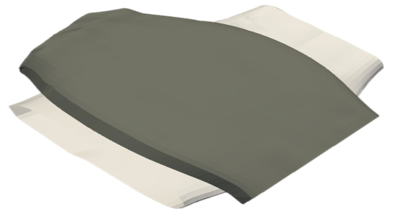
\includegraphics[width=.8\linewidth]{Close_Tows.png}
  \caption{Two Tow Surfaces in Close Proximity}
\end{subfigure}

\begin{subfigure}{.6\textwidth}
  \centering
  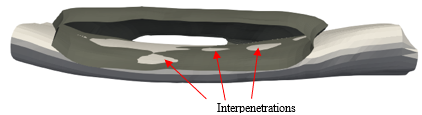
\includegraphics[width=.8\linewidth]{Penetrating_Tows.png}
  \caption{Through View of Penetrating Tows}
\end{subfigure}
\caption{Tow Surface Illustration and Penetrations}
\label{fig:fig}
\end{figure}

\section{VTMS Surface Representation Types}

VTMS has two distinct data types for its surface representations. They will be discussed below.
\subsection*{VTMS' Standard Tow Format}
Once the yarn bundles are approximated as a surface, VTMS stores this surface as a standard tow format. Internally in the software, this data structure stores surface node coordinates and normals, along with stacks that define the cross-section of the surface along the tow path. Also internally stored are surface elements that connect surface nodes and are used for visualization purposes. However, once this data is exported to a file, only node location, node normal, and which stack the nodes belong to is stored. This effectively reduces the usefulness of the data when exported. 

\subsection*{VTMS' Clipped Tow Format}
Once the surface representations in VTMS are clipped to a desired dimension, the surface data is transformed into the clipped tow format. The clipped tow format is similar to many finite element mesh representations. When exported to a file, the data is organized into node location information, surface element type, and the connectivity of the surface elements by referencing node number. The file also stores the outward normal of each surface element. The internal representation of this data is similar to the exported representation and there is much less information lost when exported. 


